\begin{frame}\frametitle{Jets$\rightarrow \gamma$ Background. Sources}
  \scriptsize
  Jets$\rightarrow \gamma$ background estimation is the most challenging part of this measurement and also the source of the largest systematic uncertainties (discussed later).
\end{frame}

\begin{frame}\frametitle{Jets$\rightarrow \gamma$ Background. Template Method}
 \scriptsize
  \begin{itemize}
    \item Choose a variable that has a significant discriminative power between the true and fake photon candidates $V_{fit}$;
    \item Prepare real-$\gamma$ ($T_{true}$) and fake-$\gamma$ ($T_{fake}$) templates {\tiny{(next slide)}};
    \item Fit $V_{fit}$ distribution in data by: $F(V_{fit})=N_{true} \cdot T_{true}(V_{fit}) + N_{fake} \cdot T_{fake}(V_{fit})$.
  \end{itemize}
\tiny
Templates: accurate representations of $V_{fit}$ distributions of real-$\gamma$ and fake-$\gamma$ in the $W\gamma$-selected dataset.\\
- - - - - - - - - - - - - - - - - - - - - - - - - - - - - - - - \\
  \begin{figure}[htb]
    \begin{center}
       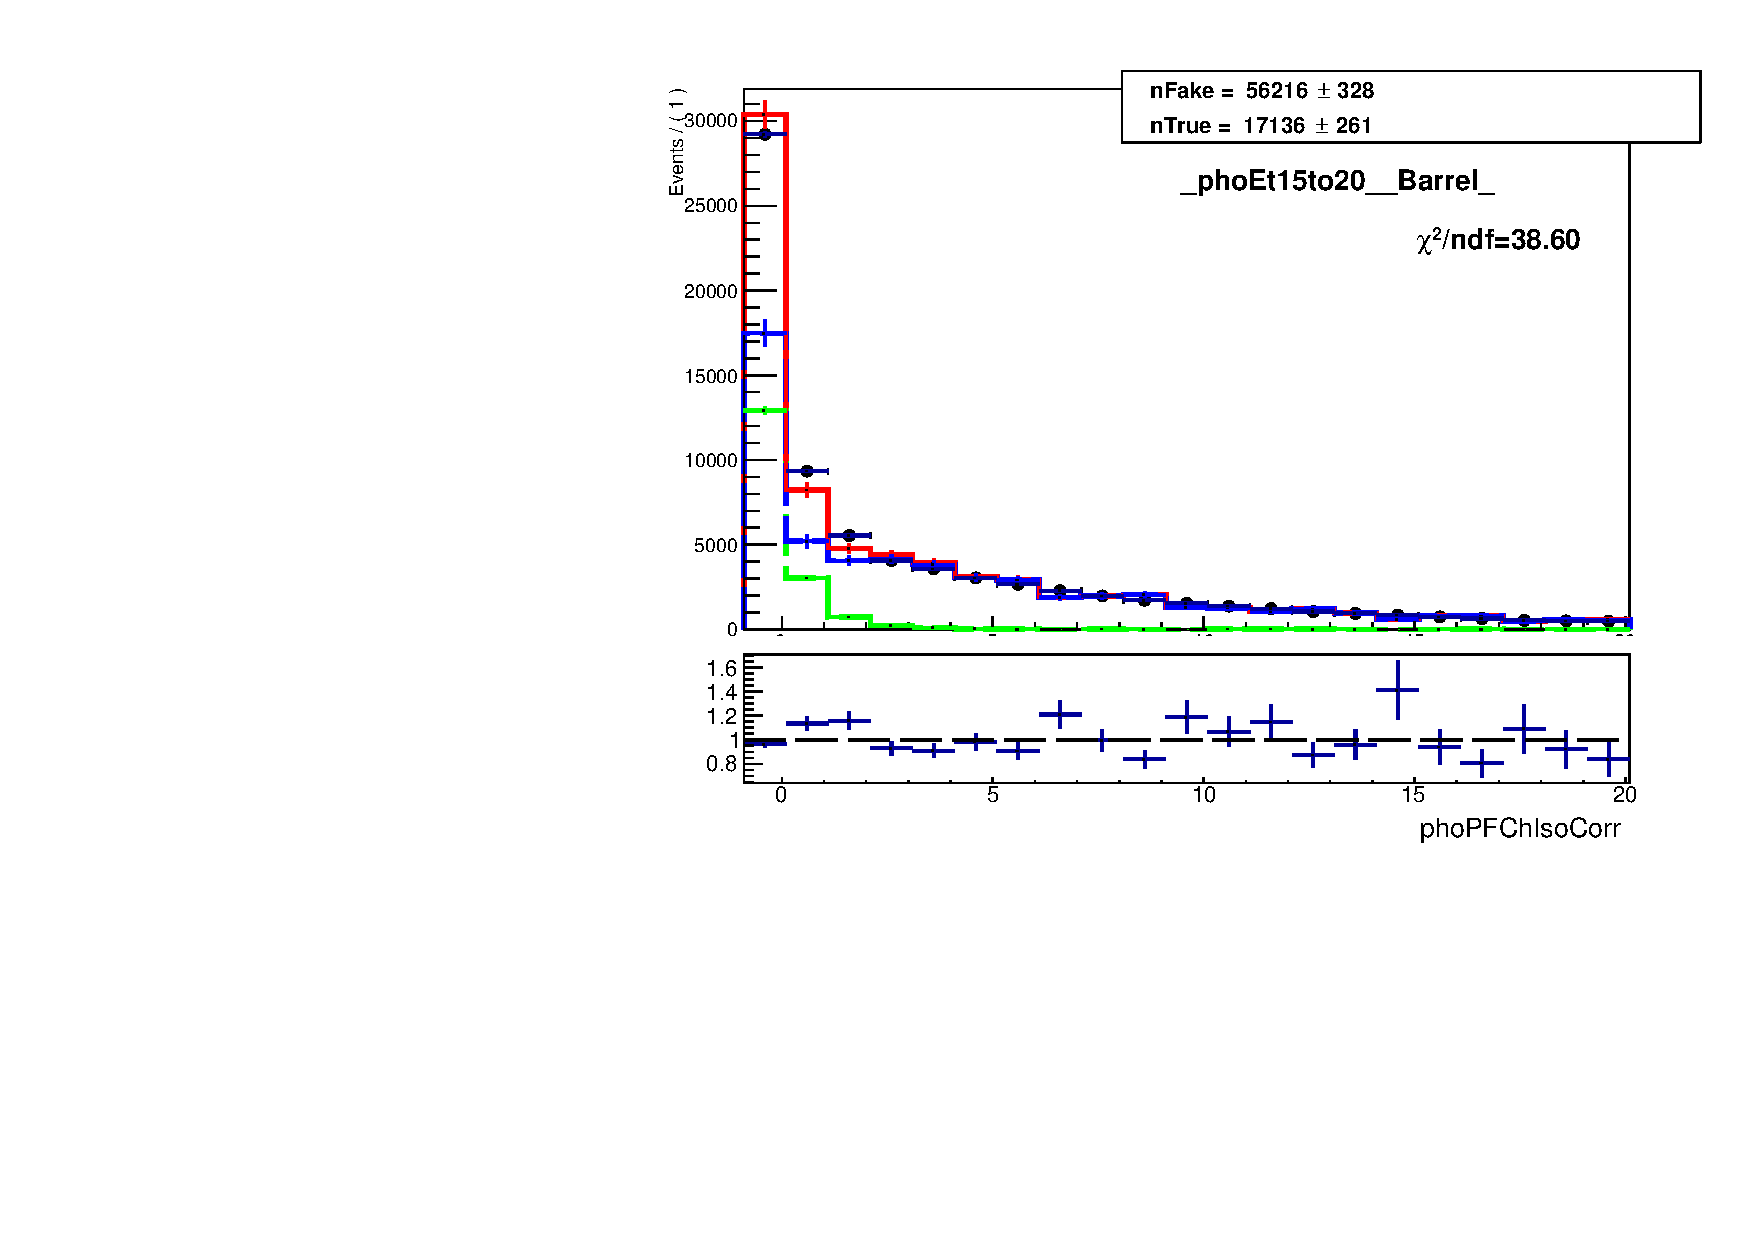
\includegraphics[width=0.40\textwidth]{../figs/figs_v11/MUON_WGamma/TemplateFits/c_TEMPL_CHISO_UNblind__phoEt15to20__Barrel__RooFit.pdf} 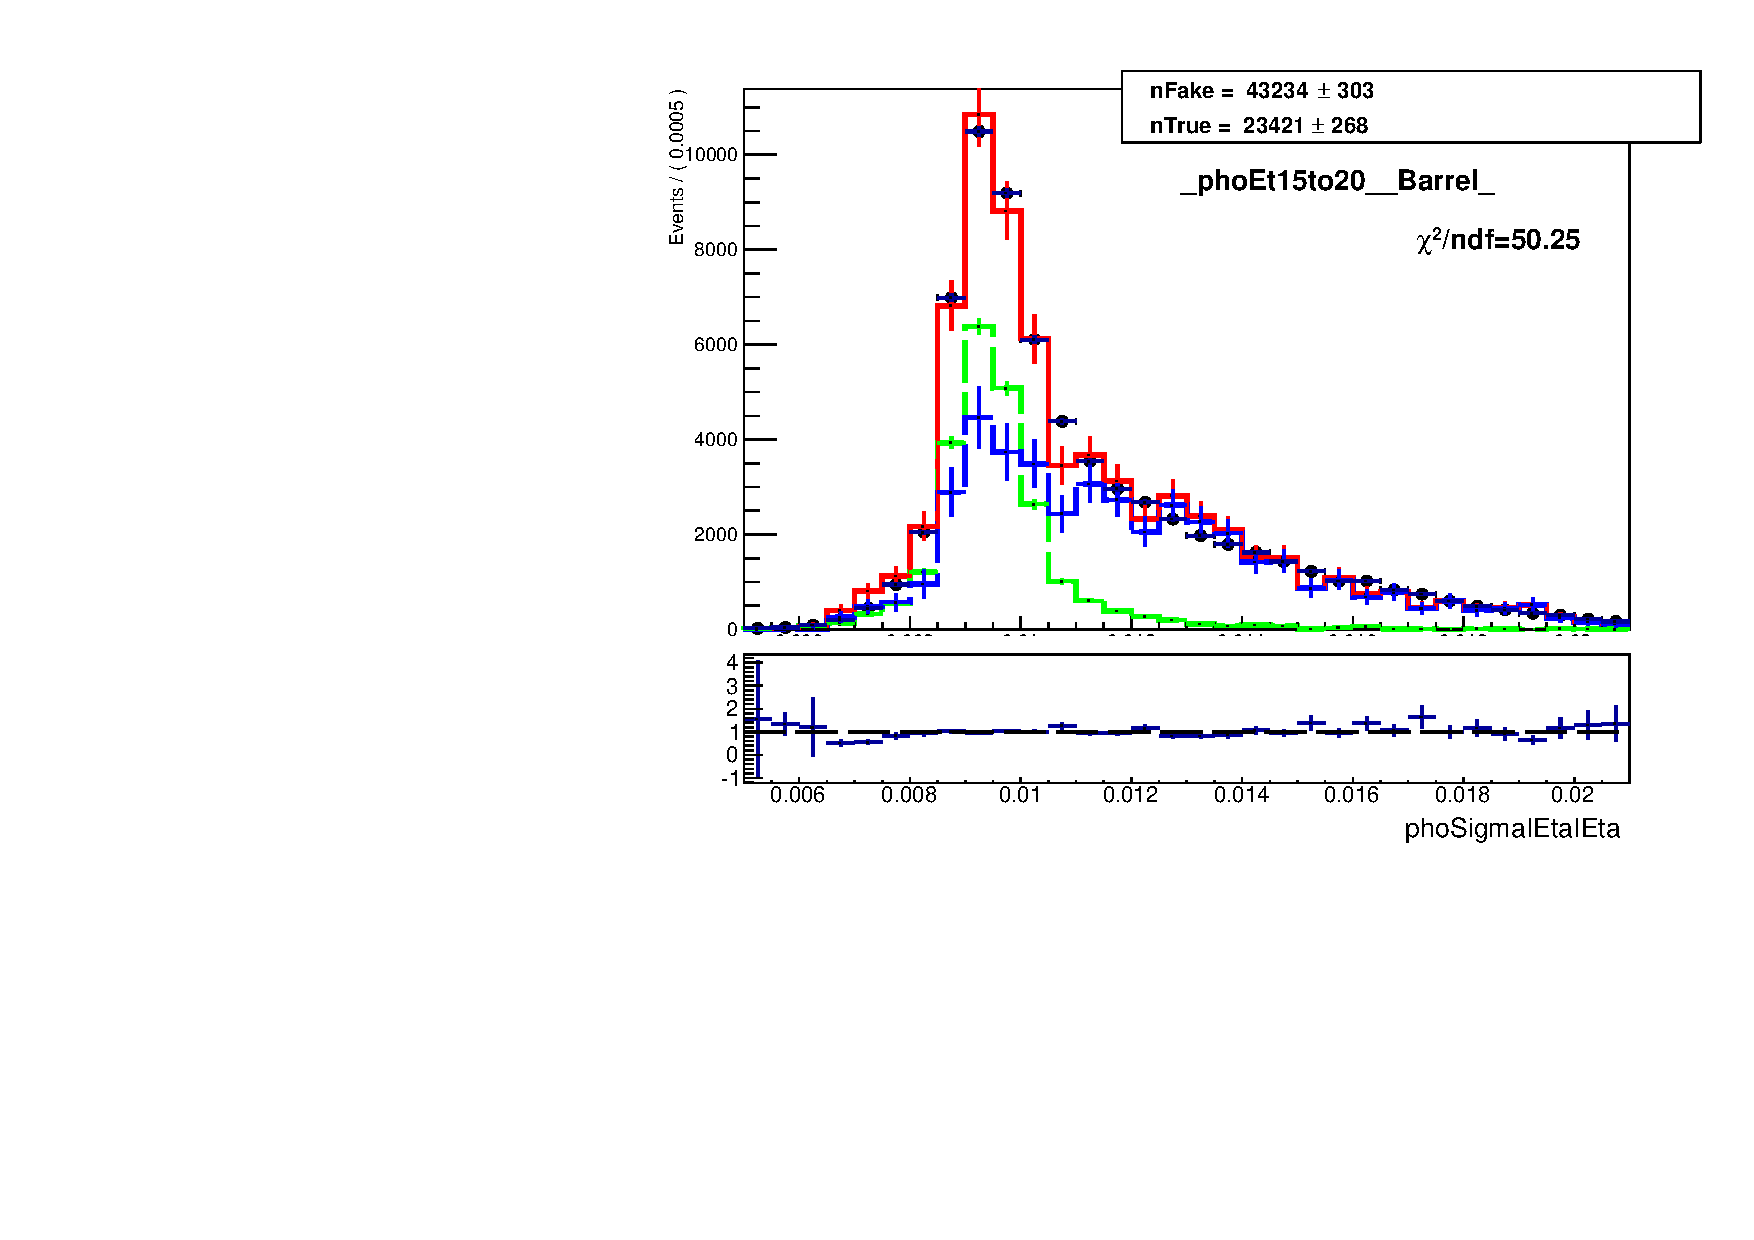
\includegraphics[width=0.40\textwidth]{../figs/figs_v11/MUON_WGamma/TemplateFits/c_TEMPL_SIHIH_UNblind__phoEt15to20__Barrel__RooFit.pdf}
    \end{center}
  \end{figure}
\scriptsize
$I_{ch}^{\gamma}$ (charged hadron isolation):  $I_{ch}^{\gamma} = \sum P_T^{ch.had.}$, $\Delta R(\gamma,$ch.had.$)<$0.3\\
$\sigma_{i\eta i\eta}$: an ECal shower shape variable\\
\tiny
{\bfseries{black}}: data; {\bfseries\color{green}{green}}: real-$\gamma$ template; {\bfseries\color{blue}{blue}}: fake-$\gamma$ template; {\bfseries\color{red}{red}}: fit function
\end{frame}

\begin{frame}\frametitle{Jets$\rightarrow \gamma$ Background. Templates from $Z\gamma\rightarrow{\bar{\mu}}\mu\gamma$}

  \begin{figure}[htb]
      \begin{center}
        \scriptsize
          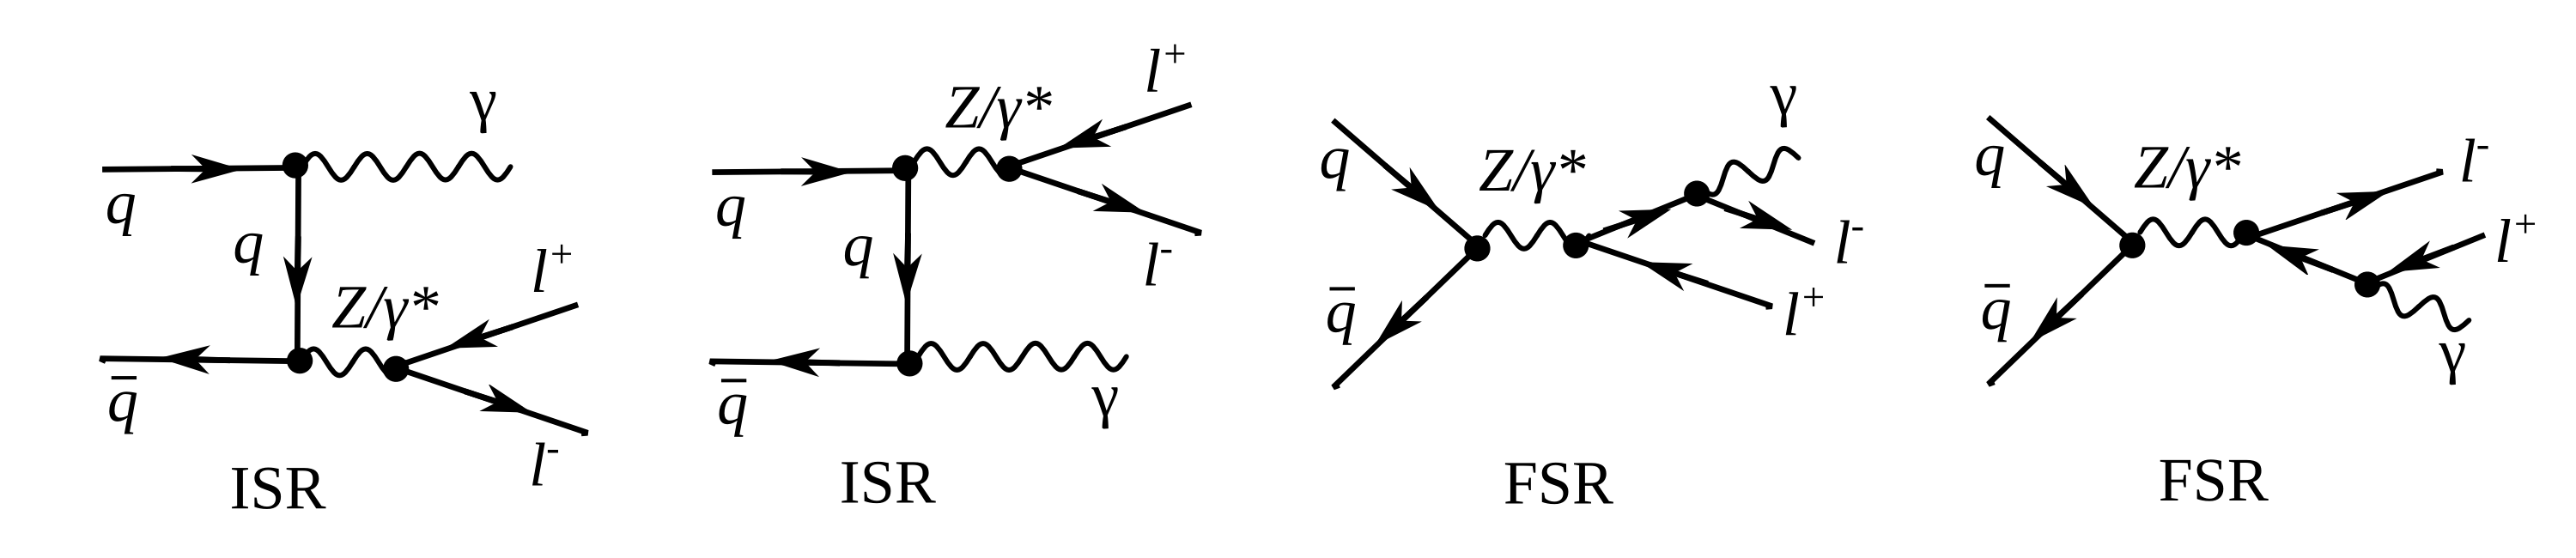
\includegraphics[width=0.95\textwidth]{../figs/ForPresentation/feynmZg_LO.png}
%          \caption{\scriptsize{The Feynman diagrams. ISR(x2), FSR, and TGC.}}
       \end{center}
    \end{figure}

\scriptsize
FSR: final state radiation; ISR: initial state radiation

  \begin{figure}[htb]
    \begin{center}
       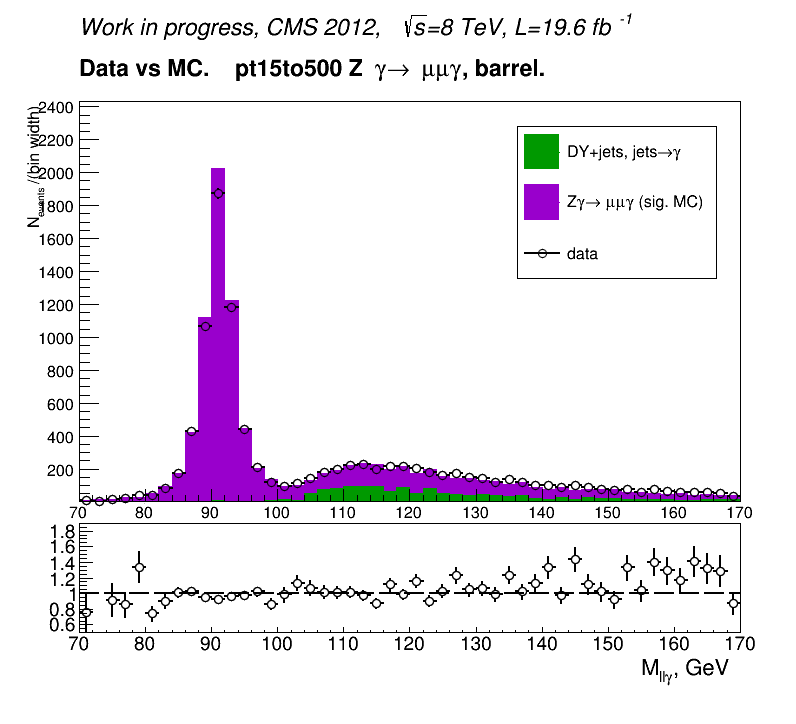
\includegraphics[width=0.40\textwidth]{../figs/figs_v11/MUON_ZGamma/PrepareYields/c_TotalDATAvsMC_Barrel__MpholeplepVERY_PRELIMINARY_pt15to500_.png}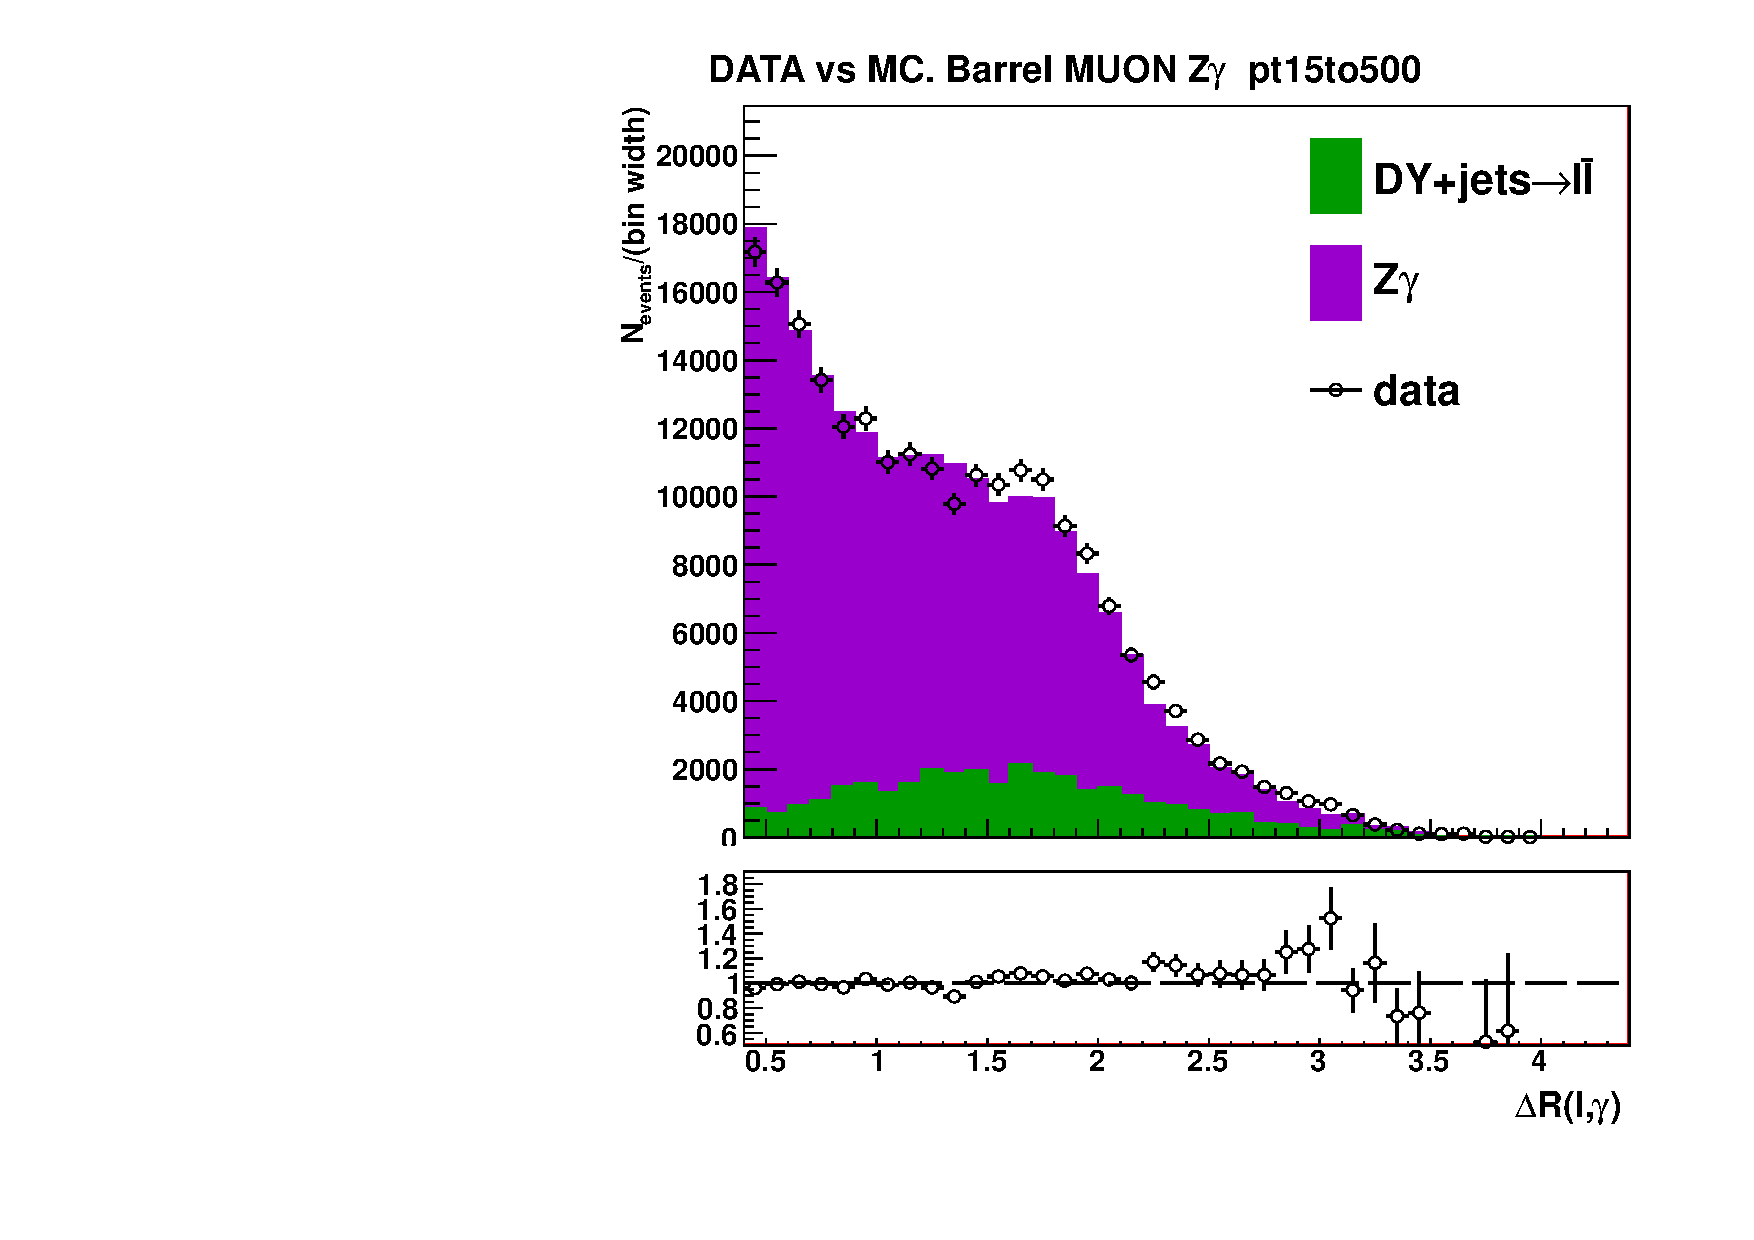
\includegraphics[width=0.40\textwidth]{../figs/figs_v11/MUON_ZGamma/PrepareYields/c_TotalDATAvsMC_Barrel__lep1PhoDeltaRVERY_PRELIMINARY_pt15to500_.pdf}\\
% 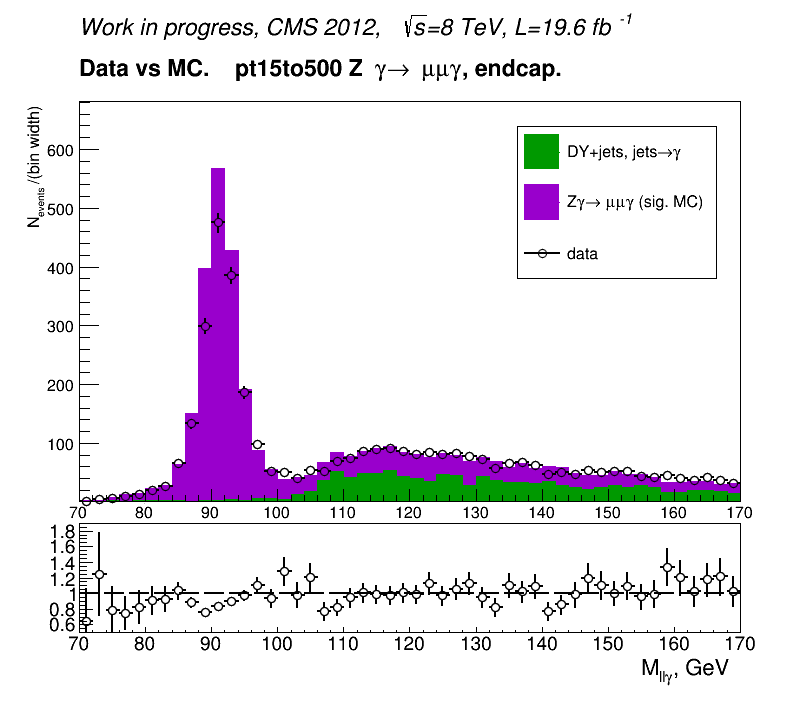
\includegraphics[width=0.40\textwidth]{../figs/figs_v11/MUON_ZGamma/PrepareYields/c_TotalDATAvsMC_Endcap__MpholeplepVERY_PRELIMINARY_pt15to500_.png}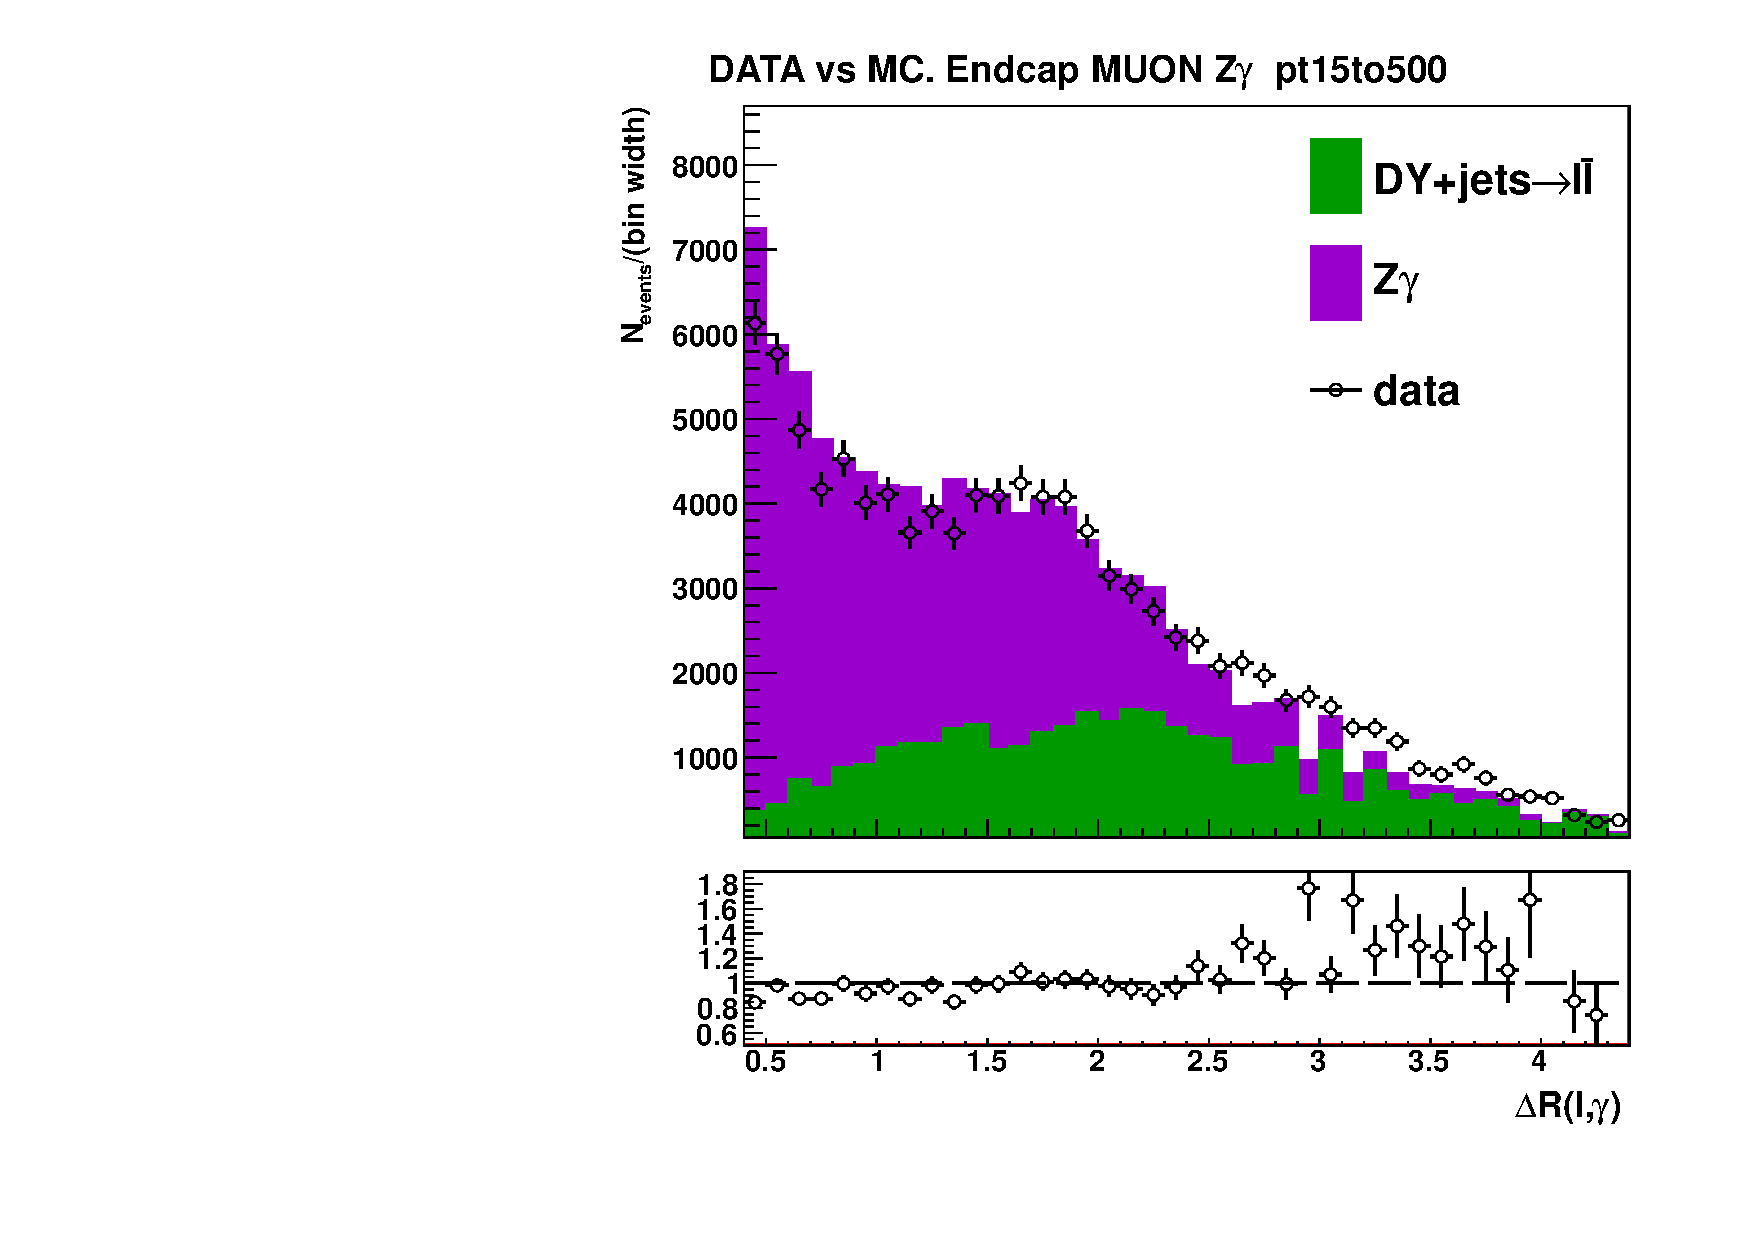
\includegraphics[width=0.40\textwidth]{../figs/figs_v11/MUON_ZGamma/PrepareYields/c_TotalDATAvsMC_Endcap__lep1PhoDeltaRVERY_PRELIMINARY_pt15to500_.pdf}
    \end{center}
  \end{figure}
\scriptsize
Increase real-$\gamma$ fraction (FSR): $M_{\mu\mu\gamma}<$101~GeV and $\Delta R(\mu_{1},\gamma)>$0.4\\
Increase fake-$\gamma$ fraction (ISR): $M_{\mu\mu\gamma}>$101~GeV and $\Delta R(\mu_{1},\gamma)>$1.0

\end{frame}%{{Jets$\rightarrow \gamma$ Background. Templates from $Z\gamma\rightarrow{\bar{\mu}}\mu\gamma$}
